\chapter{Motivation}

\begin{flushright} 
%\textit{"Begin at the beginning and go on till you come to the end: then stop."
%\\-Lewis Carroll, Alice's Adventures in Wonderland.}\end{flushright} 
\textit{"An approximate answer to the 
right problem is worth a good deal more 
than an exact answer to an approximate problem." \\
- John Tukey}\end{flushright} 
\begingroup
\textit{Our everyday lives get more and more saturated with computing devices and embedded in them, a wide variety of sensors. With access to powerful computing, sensors and a ubiquitous Internet, why is context recognition, and with it pervasive computing, not further along and more broadly adapted? With few exceptions, most context recognition research done to date assumes dedicated sensing devices with fixed locations. These locations are often carefully chosen to suit a particular application. This is a major limitation hindering broad adoption of pervasive computing systems. Who wants to bother to put on a second "sensor suit" before leaving to work in the morning or re-adjust shifted sensors every couple of hours? Is there a way to deal with device placement and orientation changes to make context sensing more mainstream?}
%\textit{
%With people having access to powerful computing devices, the Internet being ubiquitous and pervasive computing concepts getting mainstream, why is activity sensing not further along and more broadly adapted?
%Our everyday lives get more and more saturated with computing devices and embedded sensors. Most notably, smart phones become an important computing platform and, in general, the quality of smart phone sensors is not much different from the devices typically used in dedicated wearable sensing systems. However, with few exceptions the bulk of
%context and activity recognition work done to date assumes known fixed sensor 
%locations which are often carefully chosen to suit a particular application.
%Mobile phones and other wearable devices, on the other hand, are
%carried by users in a variety of locations. In most cases they are not firmly
%fixed to the body but placed in a pocket or bag where the can shift around and have different orientations. This chapter sets the stage, exploring the state of the art in activity sensing with a focus on on-body context recognition, discussing challenges, potential obstacles.}
%This thesis presents a systematic evaluation of device
% placement effects in activity recognition. A categorization of the
% placement factors concerning context recognition systems is
% proposed. We present a systematic evaluation of these device
% placement factors on common sensing modalities,
% used in activity recognition today. In the course of
% the thesis, we introduce methods to infer the symbolic placement of a
% device and approaches to deal with coarse grain and fine variations
% in placement. This motivation chapter gives a small introduction
% into the current state of activity recognition. According to an
% assessment using two user studies, two important requirements are
% sensor integration into every day objects and device placement
% independence. As those two requirements are the basis for this
% thesis, research related to them is discussed. After the
% introduction in the field, Sections~\ref{aims},~\ref{contributions}
% and \ref{mot:overview} present the aims, contribution, outline and
% overview of this thesis in relation to the state of the art in
% research.}
%\\\\ Kunze, K.,
%Wagner, F., Kartal, E., Morales Kluge, E., and Lukowicz, P. Does
%Context Matter ? - A Quantitative Evaluation in a Real World\vskip\onelineskip
\vskip\onelineskip
\begin{adjustwidth}{}{-\chapindent}%
\hrulefill 
\end{adjustwidth}\endgroup
\vskip\onelineskip
\vskip\onelineskip 
%Pervasive computing has grown up. Today, we rely more and more on the
%ubiquity of sentient objects in our everyday life with the smart phone
%becoming an important computing
%platform~(\cite{Chronis:2009p7854,Krause:2006p1884,Ofstad:2008p7556,Choudhury:2010p5381,
% hinckley2001tms}). 
%\noindent As we use computers more and more to assist us in our daily activities, the amount
%of RAM, CPU speed etc. are no longer the limiting performance factors.
%The bottleneck becomes human attention. To overcome this limitation, pervasive
%computing tries to minimize direct user interaction. Computing systems
%are to become pro-active, inferring user intent (\cite{tea}). Context
%recognition is considered a fundamental concept in pervasive computing. 
%Activity recognition today is realized using sensors on the user's body and in
%the environment. Utilizing these sensors computer systems perceive the
%user's actions and are, therefore, able to support the user pro-actively.
%The tech industry acknowledges the pervasive computing idea and
%embraces context-aware computing as a significant
%innovation. TechCrunch - a company offering news around high-tech and
%web start-up names "Context-Aware Apps" as one of 7 most important
%technologies for 2011 and describes them as follows:
Pervasive Computing has matured. Today, we rely more and more on computing devices to help us in our daily activities, with the smart phone becoming an important platform~\cite{Chronis:2009p7854,Krause:2006p1884,Ofstad:2008p7556,Choudhury:2010p5381,hinckley2001tms}. As these devices --and with them computing-- become tighter integrated in our everyday lives, the performance bottlenecks, even on mobile platforms, are no longer RAM capacity, CPU speed etc. We use computing more and more in environments in which we cannot focus our attention completely on the device in question (e.g. during our daily commute, while waiting in a queue, during lectures/meetings). In these situations, human attention is sparse. It becomes the crucial bottleneck.

For the user to be able to interact with computer systems even in "busy" environments, 
%To levitate the user of the burden to directly interact with more and more computer systems, 
pervasive computing introduces context recognition as a core concept~\cite{tea}. 
Context recognition infers relevant information about the current situation of the user utilizing sensors carried on the body and distributed in the environment.
This information, the user's "context", helps to minimize direct user interaction. Pervasive applications adjust their behavior pro-actively according to the given situation.

Context recognition is not just a theoretical concept introduced by the research community.
The tech industry also embraces context-aware computing (computing utilizing context recognition) as a game changer. TechCrunch, a company offering news around high-tech and web start-ups, names "Context-Aware Apps" as one of 7 most important technologies of 2011 and describes them as follows:

\begin{quote}
\textit{"Context-Aware Apps: Whether it's search, mobile, or social apps and
services, the most useful apps people will keep coming back to are the
ones which help people cut through the increasing clutter of the
Internet. Apps that are aware of the context in which they are being
used will serve up better filtered information... %When you search on
%your mobile phone, that means you get local results and local offers
%served up first...
%If you are on a service like Quora that understands
%your interest graph, it means that you are only shown topics that you
%care about, sorted in realtime. If you are on a news site, you will
%see the most shared links from people in you follow on Twitter or are
%connected to on Facebook. Music and movie services will similarly
%surface social recommendations. 
In a world of information overload, context is
king."}~\footnote{http://techcrunch.com/2011/01/02/seven-technologies-that-will-rock-2011/} \end{quote}

%Activity recognition matures slowly from being a mere lab curiosity
%towards becoming a technology used every day in the real world.


Companies not only acknowledges pervasive computing, some products already 
adopt pervasive computing concepts with a focus on context recognition technologies. Foremost, location-based services gain more and more momentum, from simple location check-ins (Foursquare, Gowalla, Facebook places etc.) over location-based reminders (Apple's Reminder App) to recommending restaurants close by (Yelp). 
Although Schmidt et. al. already realized in 1999 that "There is more to context than location"~\cite{Schmidt:1999hn}, it took a while for services and applications to utilize other sensing modalities. The first products with notable commercial success just emerged over the last years, for example the Nintendo Wii, a gaming console using inertial motion sensors, and Fitbit~\footnote{http://fitbit.com/}, acceleration and air-pressure sensors embedded into a clasp that records steps taken, stairs climbed and simple modes of locomotion. Although these products are already useful and a commercial success, they seem to apply quite simple context recognition algorithms (e.g., the Nintendo wii remote uses thresholding on the acceleration intensity levels to detect specific motions). How much better could we get employing more complex context recognition approaches, already well established in the pervasive computing research?

%Although Schmidt et. al. titled a paper "There is more to context than
%location"(~\cite{Schmidt:1999hn}) as early as 1999, there are still
%very little services and applications utilizing other sensing
%modalities apart from location services. Some notable exceptions with
%commercial success are the Nintendo Wii, a gaming console using
%inertial motion sensors, and Nike+~\footnote{http://nikeplus.com/}, a
%accelerometer sensor embedded into a shoe counting steps. The user
%experience for both products is very pleasant; still, they lack polish
%in one important aspect. Astonishingly, they seem to apply very
%simple algorithms for gesture/step recognition, namely thresholding.
%It matters, for example, which way the Nike+ sensor is attached to the shoe. 
%If embedded upside down, the sensor will not work as advertised. 
%The sensor is orientation sensitive. Similar
%can be said about the Nintendo wii remote, the device cannot really
%verify complex movements. It will also react to simple shakes with
%correct direction and timing. One major reason for the lack of complex
%use cases seem to be that accelerometer and other sensor data is
%harder to interpret than GPS data. 

Common sensing modalities in pervasive computing include motion (acceleration, angular velocity) and sound. Generally, we cannot expect a developer with no background in signal processing or pervasive computing to figure out the user's context from raw accelerometer or sound data. For example, it is more difficult to infer the modes of locomotion from accelerometer data than the user's location from a given GPS fix. This is foremost due to the GPS "raw data" being closer to the contextual information, e.g. getting the user's location and shops/buildings in his immediate surrounding is easy using Google Maps, Openstreet Map or similar services, once we have a GPS fix. Additionally, the software support for location services is better on most platforms. Therefore, better APIs and software libraries for other sensing modalities are needed and in the process of being built. However, the main issue, why pervasive computing research is not more broadly adopted, lies somewhere else.
 With few exceptions (e.g.~\cite{lester2006par}) the bulk of context and activity recognition research assumes known fixed sensor locations often carefully chosen to recognize specific tasks (e.g. \cite{Ogris:2008p7906,Antifakos:2002p8030}). Therefore, for each application, the user has to put specific sensors at certain well-defined positions on his body or in the environment. Yet, it is unrealistic to expect this from the user for a more widespread use of pervasive systems. The burden placed on the user is too high. While the user is on the move, he is sometimes in highly augmented environments with a lot of contextual information from smart object. Sometimes, in places with little or no infrastructure, the user needs to rely on the smart objects carried on his body. The best we can realistically expect in terms of context sensing is that at any given point in time the user carries a more or less random collection of sensor enabled devices (mobile phone, watch, headset etc.) on different body locations, eg. in his pockets, bag, wrist. To reach a more wide spread adoption of context recognition applications, we should utilize these user-owned, sensor-enable devices. However, is it even possible to use these device sensors to infer information about the user's situation? Generally, the quality of these built-in sensors is not much different from sensors typically used in dedicated wearable sensing systems. Thus, for example, the iPhone features the LIS302 acceleration sensor, which has also been widely used in wearable context recognition \cite{Chronis:2009p7854,Krause:2006p1884,Ofstad:2008p7556,Choudhury:2010p5381}. Sampling rates and AD conversion accuracies are also comparable.
 
Mobile phones and other smart devices, however, are carried by users in a variety of locations \cite{Ichikawa:2005p6295}. 
In most cases they are not firmly fixed to the body but placed in a pocket or bag where the can shift
around and change orientations frequently. Not only is the on-body location unknown, the devices are also moved out of place over time. 
Of course, shifting sensors during long term deployment is also a -- mostly ignored-- issue for dedicated wearable sensing systems.

This thesis describes approaches and methods to deal with exactly these issues of changing sensor locations, shifts in orientation and displacements.
As such my research narrows the gap between the need for context-aware applications and the practical problems, encountered when trying to implement them in real life. 

The next section discusses the current research landscape in pervasive computing with a special focus on orientation and placement independence, followed by a detailed related work discussion centered around the contents of this thesis. The chapter ends with a detailed description of the contributions and an outline.

%Additionally, to reach a more wide spread adoption of activity recognition applications, we can utilize 
%user-owned, mobile appliances. Most of them come already equipped with sensors.
%In general, the quality of these sensors is not much
%different from the devices typically used in dedicated wearable
%sensing systems. Thus, for example, the iPhone features the LIS302
%acceleration sensor, which has also been widely used in wearable
%context recognition \cite{Chronis:2009p7854,Krause:2006p1884,Ofstad:2008p7556,Choudhury:2010p5381}. 
%Sampling rates and AD conversion accuracies are also similar (the accelerometer sensor in the iPhone
%can be sampled at up to 100Hz).However, there is one major difference. With few exceptions (e.g.~\cite{lester2006par}) the bulk of
%context and activity recognition work done to date assumes known fixed sensor 
%locations that is often carefully chosen to suit a particular application (e.g. \cite{Ogris:2008p7906,Antifakos:2002p8030}). 
%Mobile phones on the other hand are carried by users in a variety of locations \cite{Ichikawa:2005p6295}. 
%In most cases they are not firmly fixed to the body but placed in a pocket or bag where the can shift
%around and have different orientations. Further, users, in several studies, expressed a large
%discontent about fixing the orientation or placement of a sensing device.
%This thesis presents a systematic evaluation of device placement effects in activity recognition.

%Before we detail the technical challenges regarding activity
%recognition, there are some other pressing issues with the pervasive
%computing vision. As described, starting in the nineties
 %pervasive computing gained more and more momentum in the research 
%community and now we see the slow adoption of these technologies
%by industry. T
% Yet, do people
%really want such a kind of technology? Does context matter? Although
%these questions are not the main focus of this thesis, they are so
%fundamental to the work presented that we address them in the
%next section.

%However, most of today's context and activity recognition systems use
%probabilistic machine learning algorithms that need extensive training
%data with exact activity labels to work. Until recently mobile
%sensing research such as activity recognition, where people's activity
%(e.g., walking, driving, sitting, talking) is classified and
%monitored, required specialized mobile devices. In addition, most
%algorithms assume fixed set of sensors with known location and
%orientation. Therefore, context and activity recognition, although
%widely used in lab settings, did not really make it into our everyday
%life, yet.


\section{State of the Art in Context Recognition}
\label{mot:sota}
%We first start with a broad overview
%of the topic, and then deal with specific related work regarding this thesis in the next section.
Context recognition is an important basis for pervasive computing.
In the early 1990s, Mark Weiser coined the terms
ubiquitous computing and calm technologies. Following his vision, computing is to transparently surround and support
us during everyday life~\cite{Weiser:1996vf,Weiser:1993hb}.
Thus, computer systems need to become \textit{pro-active}. To support the user in any given situation, computing needs to be
able to "perceive" the real world. The means to achieve this are summarized
in the term "context recognition".  For a more detailed discussion on "Context" and some more formal definitions see Dey et. al. and Schmidt et. al.~\cite{Salber:1999uj,Schmidt:1999ut}.

%\begin{figure*}[t]
%\centering \includegraphics[scale=0.60]{activityrec.pdf}
%\caption{Activity recognition as an enabling research area for
%pervasive computing and related disciplines.}
%\label{fig:activityrec}
%\end{figure*}

Context recognition, today, developed into an interdisciplinary field
building on embedded systems, signal processing, machine learning,
statistics and artificial intelligence. Since context sensing is a core concept of pervasive computing, 
there exists a vast body of research. As such, there are many ways to provide a structural overview about the field.
In the following, three possible categorizations of the research and their relations to the thesis topic are discussed in , 
namely inference type, sensing modality and infrastructure vs. on-body sensing.

 
%After the concepts "ubiquitous computing" and "calm technologies" %
%were defined, several related disciplines appeared: pervasive
%computing, ambient intelligence, wearable/normadic/affective computing.
%Everyone of them comes with their own flavor, yet they
%share most of the goals explained in the paragraph on top,
%with ubiquitous computing and pervasive computing being the
%most general terms. Yet, more important, all of them share activity recognition 
%as their foundation.

\begin{description}
 \item{Infrastructure vs. on-body sensing} -- 
Continuing the initial work of Mark Weiser, researchers
first focused on infrastructure sensing, building pervasive
rooms using stationary devices (e.g. fixed cameras, microphone arrays) as sensory inputs \cite{Dimakis:jr,Pentland:1996wt}.
Installation costs and the lack of significant applications 
hindered a wide adoption in everyday life. Most room features
were nice to have (e.g. automated access and capture), yet not crucially important.
Today, there are some efforts to make infrastructure sensing available
to the masses. Patel et. al. shows interesting research using the power line
as sensor, to detect the type of electronic devices in use and to utilize it as RFID reader \cite{Patel:2007vxa,Patel:2009bi}.Complementary to the infrastructure sensing approach is research focusing on on-body activity sensing. In on-body sensing, we use devices carried or worn by the user as sensory inputs
\cite{bao2003physical}. A major advantage of this type of sensing is it "follows" the user, as he carries the system with it. On the other hand, to carry around dedicated
sensing devices places an additional burden on the user. These devices can be annoying and heavy, especially regarding early wearable research prototypes.
Often, multiple accelerometers positioned on the users' body are used to support diverse applications, from a
meeting annotation tool to motion analysis in sports.
\cite{kern2003multi,mantyjarvi2001recognizing,ZHANG:2004wa}. Sound, in an on-body sensing scenario, can be used to infer a particular room the user is in, distance between devices and even some distinct activities (e.g. the use of a coffee grinder)~\cite{Stager:2007wm,Wyatt:2007ta}. 
There are also more and more hybrid approaches combining infrastructure and on-body sensing. In this case, on-body sensors interact with devices in the environment. The most developed context type in this aspect is location. For a more detailed discussion of different location sensing approaches, including relative and absolute positioning, please refer to Section 2.1. 

\item{Sensing modality} -- %The number of modalities is as vast as the distinct application cases of context sensing. 
Common sensing modalities in early work include
mostly sound and vision, yet also acceleration is very prevalent. 
The simplest sensors used in activity recognition are binary. They produce
only an activation signal, e.g., RFID readers/tags and ball switches.
More sophisticated experimental setups integrate
motion sensors (accelerometers, gyroscopes and magnetic field sensors
combined), force resistive sensors, sound and a location system to detect
activities from fine-grained work steps at a car assembly to 
food intake gestures~\cite{Ogris:2008p7906,Amft:2009ir}. 
Context recognition also includes some more exotic sensing modalities,
from eye movement capture using electrooculography to emotional state
detection over galvanic skin response~\cite{Bulling:2008dz,Westeyn:2006ik}. 
It is often difficult to pick the correct modality for the application task at hand. 
So far, researchers rely heavily on experience.
\item{Inference type} -- The kind of context recognition algorithms used ranges from
simple thresholding over frame-by-frame recognition approaches
to sophisticated time-series algorithms~\cite{bao2003physical,Ogris:2008p7906}. 
Inference often follows
a chain. Close to the raw sensor data, embedded systems and signal processing
methods are applied, followed by one or several machine learning/artificial
intelligence approaches. These, in turn, utilize some specific knowledge
encoded from the given application domain. A very popular research topic is also the 
fusion of different sensor modalities using specific inference types, namely feature and classifier fusion (and hybrid approaches). For an introduction to this topic see Ruta et. al.~\cite{ruta-overview}.
\end{description}

%\begin{sidewaystable}
% \caption[State of the art in activity recognition]{Exploring activity recognition research along the two dimensions: sensing modality and inference type.
%We present the reference and the name of the first author, as well as the application domain activity recognition
%is applied to in their respective research.}
% \centering
%\noindent
%\setlength{\extrarowheight}{5.5pt}
%\begin{tabularx}{ \textwidth}{ c| c c c c c c }
%\toprule[1.5pt]
%\parbox[t]{3.5cm}{Sensing Modality/\\ Inference Type}& Binary& Motion& Sound& Vision& Capacitive &Multiple\\
%\midrule[1pt]
%Thresholding-Raw & Langheinrich\cite{Langheinrich:2000vb} &Siewiorek\cite{1241422} & & & & \\
% & Groceries & Activity levels&- & -& - & -\\
%\midrule
%Frame-by-frame &Gordon~\cite{5665861} & Bao~\cite{bao2003physical}&St\"ager\cite{Stager:2007wm}&Kerhet\cite{DBLP:journals/jrtip/KerhetMLBB07} &Cheng\cite{DBLP:conf/pervasive/ChengAL10} &Ward\cite{springerlink:10.1007/978-3-540-24646-6_2}\\
%&Office work & Locomotion &Assisted Living &Movement &Swallowing &Workshop\\
%\midrule
%Time series & Taipa ~\cite{springerlink:10.1007/978-3-540-24646-6_10}&Westeyn\cite{10.1109/ISWC.2005.45} & Wyatt\cite{Wyatt:2007ta} &Starner\cite{starner1998vca} &Amft\cite{Amft:2009ir} & Ogris\cite{Ogris:2008p7906}\\
%& Household & Autistic Behaviour& Social Dynamics &Overview &Food intake &Assembly\\
%\midrule
%Hierarchical& Patterson\cite{Patterson:2005:FAR:1104998.1105283}&Huynh\cite{Huynh:2008:DAP:1409635.1409638} &Choudhury\cite{Choudhury:2002:BSL:839291.842788}&Andriluka\cite{4587583} & &Bannach\\
%& Daily routine& Daily routine &Conversations& People&- &Breakfast\\
%\bottomrule[1.2pt]

%\end{tabularx}
%\label{table:activity}
%\end{sidewaystable}

\begin{table}
 \caption[State of the art in activity recognition]{Exploring activity recognition research along the two dimensions: sensing modality and inference type.
We present the reference and the name of the first author, as well as the application domain activity recognition
is applied to in their respective research.}
 \centering
\noindent
%\setlength{\extrarowheight}{5.5pt}
\begin{tabularx}{ \textwidth+5pt}{ c| c c c}
\toprule[1.5pt]
\parbox[t]{3.5cm}{Sensing Modality/\\ Inference Type}& Binary& Motion& Sound\\
\midrule[1pt]
Thresholding-Raw & Langheinrich\cite{Langheinrich:2000vb} &Siewiorek\cite{1241422} & \\
 & Groceries & Activity levels & \\
\midrule
Frame-by-frame &Gordon~\cite{5665861} & Bao~\cite{bao2003physical}&St\"ager\cite{Stager:2007wm}\\
&Office work & Locomotion &Assisted Living\\
\midrule
Time series & Taipa ~\cite{springerlink:10.1007/978-3-540-24646-6_10}&Westeyn\cite{10.1109/ISWC.2005.45} & Wyatt\cite{Wyatt:2007ta}\\
& Household & Autism& Social Dynamics\\
\midrule
Hierarchical& Patterson\cite{Patterson:2005:FAR:1104998.1105283}&Huynh\cite{Huynh:2008:DAP:1409635.1409638} &Choudhury\cite{Choudhury:2002:BSL:839291.842788}\\
& Daily routine& Daily routine &Conversation\\
\bottomrule[1.2pt]
\end{tabularx}

\begin{tabularx}{ \textwidth}{ X c }
 & \\
\end{tabularx}

\begin{tabularx}{ \textwidth+5pt}{ c| c c c}
\toprule[1.5pt]
\parbox[t]{3.5cm}{Sensing Modality/\\ Inference Type}& Vision& Capacitive &Multiple\\
\midrule[1pt]
Thresholding-Raw & & & \\
 & -& - & -\\
\midrule
Frame-by-frame &Kerhet\cite{DBLP:journals/jrtip/KerhetMLBB07} &Cheng\cite{DBLP:conf/pervasive/ChengAL10} &Ward\cite{springerlink:10.1007/978-3-540-24646-6_2}\\
&Movement &Swallowing &Workshop\\
\midrule
Time series &Starner\cite{starner1998vca} &Amft\cite{Amft:2009ir} & Ogris\cite{Ogris:2008p7906}\\
&Overview &Food intake &Assembly\\
\midrule
Hierarchical &Andriluka\cite{4587583} & &Bannach\cite{Bannach:2010wt}\\
& People Tracking&- &Morning Routine\\
\bottomrule[1.2pt]

\end{tabularx}

\label{table:activity}
\end{table}


%As already mentioned, we will not deal in particular with the on-body vs.
%infrastructure category, as the theme of this thesis focuses on on-body sensing.
This thesis centers on on-body sensing, although some of the presented approaches 
 work very well in an infrastructure setting, especially the active sampling method in Chapter 2.

To review the current state of context recognition
we will explore recent research along the two other categories:
sensing modality and inference type. Table~\ref{table:activity} gives
an overview. We center on some highlights from this summary  
moving along the sensor modality axis first and the inference type second, starting with "binary" for "raw/thresholding" inference, over motion, sound, vision, capacitive to multiple. For each sensing modality, we first look at relative simple inference types from raw over frame-by-frame to more complex time series and hierarchical approaches.

"Binary" regarding the sensor modality stands for the granularity of the sensor resolution.
The sensor can only distinguish activation versus no activation, e.g. a switch sensor integrated in a cupboard door emits either "door opened" or "door closed". Langheinrich et. al. provide an excellent example for
the simplest inference type using the raw signal from binary sensors~\cite{Langheinrich:2000vb}. 
They use RFID tags embedded in consumables bought in the supermarket. The bought products are match against recipes and the user receives recipe suggestions. Moving to the frame-by-frame inference type, 
features are usually calculated on the sensor data over a sliding or jumping window.
These are then used to do a frame-by-frame classification with standard
machine learning algorithms (e.g. KNN, desicion trees). 
Gordon et. al. show how to utilize simple binary ball switches 
as an interesting alternative to accelerometers. The new design
presented in the paper is very small (2 x 3 mm) and works
well for high frequency movements~\cite{5665861}. Although they
deliver only binary information, the initial analysis on an office
data set indicates that they can also be used
as a complementary sensor to accelerometers due to their ability to
capture high frequency components. Combining both increases the overall accuracy. 
Van Laerhoven et. al. present a comparison between traditional ball switches and
accelerometers~\cite{laerhovengellersen2004}. They use multiple ball switches
in several orientations to compensate for the information loss 
compared to an accelerometer. 

Motion in general and the accelerometer in particular is a very prominent sensing modality
used in context recognition. Siewiorek et. al. present
a mobile phone platform that can log the users activity levels 
during everyday activities, using simple thresholding on the acceleration norm. Very early work from Bao used the
frame-by-frame classification approach to detect  modes of locomotion: walking, standing, sitting etc.~\cite{bao2003physical}.
Frame-by-frame classifiers work well on context types that are repetitive in nature (e.g., walking). 
Using time-series approaches is relatively common for more complex activity recognition 
based on motion. Mostly Hidden Markov Models and Conditional Random Fields are applied.
Westeyn et. al. introduce a system that assesses the risk for autism in toddlers \cite{10.1109/ISWC.2005.45}. 
They integrate motion sensors into toys, recognizing specific repetitive gestures indicative of autism.
The recognition results are used to store and augment a video for later expert review. 
The application scenarios for motion based inference are pretty wide and range from daily routine over furniture assembly to car manufacturing,
usually a combination of frame-by-frame, time series and hierarchical inference methods is applied to reach satisfactory recognition results  in realistic application scenarios~\cite{Antifakos:2002p8030,Ogris:2008p7906}.

A good reference for sound-based context recognition is research by St\"ager et. al. 
\cite{Stager:2007wm}. They present an approach evaluated on low power special
purpose hardware, optimizing power consumption
and recognition rate. Both of them are obviously competing goals. 
Given the needed accuracy and the power constraints, their method enables to find
the best trade-off. The application scenarios shown are kitchen work and, more
general, assisted living. 
Very interesting work using sound and higher level inference methods
comes from Wyatt et. al.\cite{Wyatt:2007ta}. They try to determine the structure and changes
in social networks by detecting face to face communication.

The use of vision in activity recognition research is sparse compared to
motion or sound, especially if we focus on on-body sensing. This is largely
due to the fact that cameras are a complex sensor type and
influenced by many noise sources (lighting, reflections etc.).
Vision inference also requires a significant amount of computing power. 
One of the few usage scenarios for vision in a wearable setting is the recognition of sign language~\cite{starner1998vca}.
An overview about the role of computer vision in activity sensing is given
by Starner et. al.~\cite{starner1998vca}. 

Using multiple sensors for inference, also called multimodal activity 
recognition, presents additional problems, as one needs to find
the means to successfully fuse them. Most work in this category uses
one sensing modality to do the segmentation of the sensor data
before the classification is performed. 
Ward et. al. use body-worn accelerometers and
microphones to recognize workshop activities (drilling, sandpapering etc.) 
using an interesting segmentation technique~\cite{springerlink:10.1007/978-3-540-24646-6_2}. 
The user wears a microphone on the
wrist and one on the torso. To recognize if an interesting event happens (i.e. the user works with this hand), 
one compares the
intensities of the two microphones. If the intensity on the wrist is higher
than a given threshold, it is very likely the sound originated from an 
activity the user performed with his hand.
Ogris et. al. follow a similar segmentation approach by filtering according to location.
They use an indoor location system to pre-select the activity class.
As many given activities can only be performed at specific locations, this
can be used to limit the set of activity candidate of the classification stage
(e.g., you wont brew coffee in your car). In addition they apply a variety
of sensor fusion methods (voting etc.) to a car assembly data set.
More detailed work related to multimodal activity recognition can be found
in Sections 2.1 and 5.2.

These categories are, by no means, meant to present a complete classification
of the context recognition field. Yet, they help to categorize this thesis.
We will center on on-body sensing using mainly motion sensors 
with a specific emphasis on novel inference algorithms and sensor fusion methods.

The integration of the more common sensing modalities in smart appliances and the
wide-spread adoption and usage of these devices opens
up new, fascinating opportunities for activity recognition, moving slowly 
from recognizing the small-scale activities of a single person 
towards inferring collective social activities 
e.g. crowd density, emotional state and enabling citizen science~\cite{Eagle:2006p1070,Aoki:2008p1188}.
We will discuss this field in greater detail in the future work section of the conclusion.

\section{Related Work}
\label{mot:relatedwork}
While there is a vast variety of context recognition applications and sensor
modalities, as seen from the examples
above, so far traditional research work follows a specific
pattern. Given an application domain, the researchers use dedicated
sensor devices hand-picked for the tasks according to intuition and experience.
 To perform context recognition, a standard procedure is to aggregate the sensor data using some kind of feature calculation e.g. a
sliding window approach. There is no standardized approach
for picking them yet. Also, the feature selection and recognition
methods often rely on specific sensor devices with fixed position and
known orientation~\cite{lukowicz2004recognizing,mantyjarvi2001recognizing,kern2003multi}.

Using these methods implies for the user to carry dedicated sensors and fixing them
at specific placements. This is impractical for a wide range of application scenarios.
Integration in existing devices and device placement
independence are two important requirements to apply context recognition in real life settings. 
Device placement independence depends highly on the sensing modality used.
Most inferences based on accelerometers depend 
on specific on-body placement and orientation, as variations of the accelerometer placement lead to 
 changes in the acceleration signal. The motion distribution on the sensor axes changes significantly even with small variations. 
Other modalities are a bit more placement independent, e.g. sound, bluetooth/wlan signal strength.
Subsequently, we discuss the specific scientific background and
state of the art towards more placement independent activity
recognition using everyday objects. To better understand how
feasible it is to use regular objects, e.g. mobile phones or keys, we
take a look at research in activity recognition, focusing 
on sensor device integration and approaches to deal with orientation
and placement independence.


\subsection{Device Placement Independence}

For the remainder of this thesis, we distinguish between three sensor
deployment changes: coarse variations, fine grain changes and device orientation changes.
Coarse variations imply a change in  the  "global
position" of the device, e.g. putting a sensing device from the table in the
pocket. Fine grain variations involve shifts within a "global position". Orientation changes refer to changes of the reference system
of the sensor (leaving its global position unchanged), e.g. turning a
sensor 180 degrees around an arbitrary axis. A more detailed classification of deployment changes
is given in the aims and contribution section later in this chapter. 
Three basic approaches to deal with device
placement changes are found in the literature:

\begin{description}
 \item{Unawareness:} The most trivial method is to not deal with device placement variations 
 at all. As soon as the user recognizes a miss-classification from
 the system, it is up to him to fix it. Most of the work cited in
 the previous section belongs into this category. 
 \item{Usage of less dependent sensors/features/algorithms:} 
 Different modalities exhibit differing degrees of susceptibility to the discussed changes. 
 A microphone is more placement independent than
 an accelerometer, for example. Exploiting this, however, relies heavily on the application
 scenario and the recognition tasks to support. 
 For example, Van Laerhoven et. al. introduce simple switch sensors and show that they are less body placement dependent than 
 accelerometers with similar recognition rates for simple activity recognition
 tasks~\cite{vanLaerhoven:2004p1442}. 

Another possibility to become more device placement independent is to use more robust features. 
One can aggregate the sensor data using features that alter less due to changes in orientation and placement. 
 For example, a feature often used in accelerometer based
 activity sensing is the norm of the acceleration vector, as it is orientation independent. Of course, introducing 
 these aggregations will generally lead to information loss. As soon as some aggregations are introduced, the recognition rates will decrease. 
To compensate this, it is common to combine different sensor modalities. Krause et. al. 
 describe such sensor fusion methods~\cite{Krause:2003p1536}.

 Variations in sensor placement and orientation 
 can be integrated in the training set, relying on the machine
 learning algorithm to abstract these. 
 Lester et. al. show how to do activity recognition, utilizing these three concepts, multiple modalities, 
 independent features and a test set with large variations~\cite{Lester:2006p856}. They use
 a small dedicated sensor board to reliably detect modes of locomotion
 in a user group (12 participants over 12 hours of data) that carried the device
 on various body locations. The inference is based on frequency features, also
 using the accelerometer norm as aggregation. Modes of locomotion, however,
 count to the very basic activities to be detected.
 Lu et. al. apply two concepts, using a robust sensing modality -sound- and again
 a data set with large variability~\cite{Lu:2009p7766}. The system is implemented
 on an iPhone and able to recognize ambient sounds common
 in daily living scenarios.


 \item{Placement and orientation inference:} 
 Most work in current
 activity recognition research is done towards orientation
 independence. There are some heuristics for accelerometer sensing to detect the vertical orientation~\cite{Mizell2003using,kern2002wearable}.
 Thiemjarus presents an approach to perform activity
 recognition device orientation independently, posing the orientation
 as a classification problem~\cite{bsn1}. She uses a dedicated device
 on the hip equipped with an accelerometer. The orientation inference 
 algorithm is trained on the different device rotations. Presented with
 a changed device orientation, it then returns a rotation matrix to
 be applied to the accelerometer data. Afterwards, an unaltered classifier
 can be used. Although an interesting
 approach, the paper only shows it working for 4 device
 orientations of a device attached to a belt. It still
 needs to be assessed how generalizable the method is. 
 Steinhoff et. al. show several methods on how to tolerate orientation
 changes and displacement effects for motion sensors (accelerometer, gyroscope and compass) in the front trouser
 pockets~\cite{deadreckoning}. They use the two heuristics described before, rest periods
 and low pass filtering in combination with principle component analysis methods (for
 comparisons) to infer the user's direction of motion. Yet, this can just be applied to
 dead-reckoning and similar applications. The closest work related to the
 displacement contribution comes from Forster et. al. presenting a
 genetic programming method for feature extraction. Although the
 method can compensate sensor displacements, it requires training
 with multiple sensors~\cite{Forster1}. Forster et. al. also introduce
 an online unsupervised classification algorithm for
 accelerometers that can deal with sensor displacements, yet the
 algorithm needs to run for the complete usage time of the sensor
 device~\cite{Forster2}. It seems to depend highly on the chosen
 activity classes and the method cannot compensate larger displacements. 
\end{description}


\subsection{From dedicated device to appliances}

Some early work from Schmidt et. al. describes device integration of sensors, to alter screen rotation
depending on how the users hold the device. In recent years, 
mobile phones are increasingly becoming the platform
of choice for context aware applications. According to industry
estimates in 2010, around 30\% of all mobile phones will be equipped
with an accelerometer. For smart phones this figure is close to
100\%. Many high end devices are also equipped with a variety of
additional sensors such as a digital compass, gyroscopes, GPS and WiFi
interface which can be used for indoor location. In addition a phone
trivially has a microphone which can be used for auditory scene
recognition. 

%In general, the quality of these sensors differs little from
%the devices typically used in dedicated wearable sensing systems.
%Thus, for example, the iPhone features the LIS302 acceleration sensor,
%which has also been widely used in wearable context recognition
%\cite{Ogris:2008p7906,Antifakos:2002p8030,Krause:2006p1884,Choudhury:2010p5381}.
%Sampling rates and AD conversion accuracies are also similar (the
%accelerometer sensor in the iPhone can be sampled at up to 100Hz).
%However, there is one major difference, the bulk of context and activity recognition
%work done to date assumes known fixed sensor locations that are often
%carefully chosen to suit a particular application
%(e.g. \cite{Ogris:2008p7906,Antifakos:2002p8030}).
%Mobile phones on the other hand are carried by users in a variety of locations
%(~\cite{Ichikawa:2005p6295}). 
 
%(~\cite{lester2006par,Chronis:2009p7854,Ofstad:2008p7556})
There is already some initial work using mobile phone as sensing devices.
Lane et. al. give a good introduction and overview about this topic~\cite{Lane:2010p580}. 
Chronis et. al. try to tackle social interactions using mobile phones, attempting to detect shifts
in habits and correlating them to events in the users life. They show
how they track political opinion in a study conducted at a dorm room at MIT 
using regular off the shelf smart phones~\cite{Chronis:2009p7854})
Mobile phones can also be used to localize the situation a user is in~\cite{Ofstad:2008p7556}.
Ofstad et. al. use audio fingerprints collected over the built-in microphone of the iPhone
to detect the semantic location of the user. 
Although Lester et. al. use dedicated hardware, their work discussed in detail in the previous section
 still contributes towards better device integration, as the sensor board is designed to be easily integrated 
in a phone~\cite{lester2006par}.
These examples, however, employ only less dependent sensing modalities, e.g. sound, bluetooth, or large
diverse training sets to deal with placement issues. 

\subsection{In Summary}

\begin{figure*}[t]
\centering 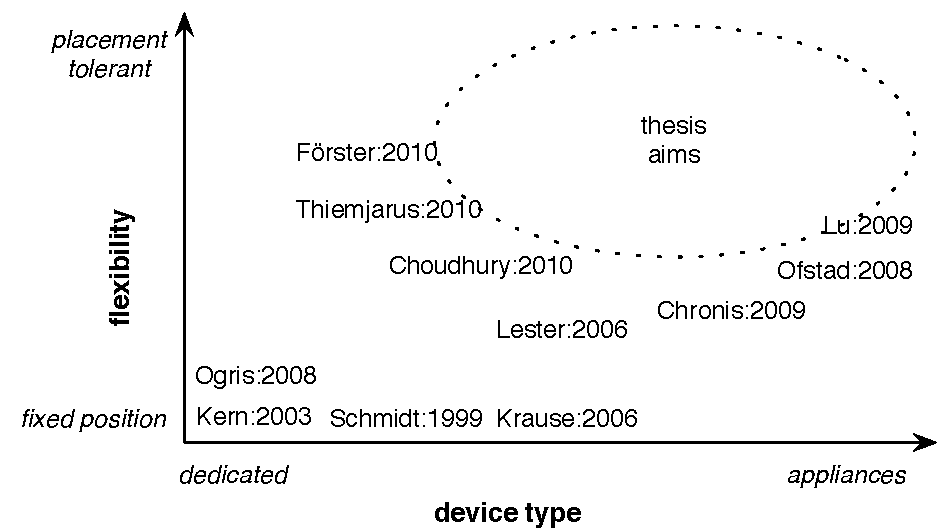
\includegraphics[scale=0.60]{related.pdf}
\caption[Related work and thesis aims]{Significant related work in relation to the aims of this
 thesis, depicted in two dimensions: flexibility (tolerant is the
 methods to displacement) and device type (dedicated sensing device
 towards integrated in everyday appliances).}
\label{fig:relatedwork}
\end{figure*}

To the best of my knowledge, there has been no detailed study about
placement effects on common activity sensing modalities. Nobody, so far,
tried to detect the on-body-positioning of devices. Providing heuristics
towards better orientation and placement independent activity
recognition is also rather unexplored, disregarding the few exceptions given in the related work. 
Figure~\ref{fig:relatedwork} depicts the current state of the art in research
in the two dimensions set by two requirements:
Placement and orientation independence (named flexibility) and 
the device integration. Although only to be taken as indication,
it summarizes the lack of research towards flexible context recognition
methods that are able to be used on commodity devices. 
Ogris et. al. use dedicated hardware without dealing with device orientation or placement changes, yet are able to 
detect very complex, large sets of activities~\cite{Ogris:2008p7906}. Foerster et. al. show
some work to deal with sensor displacement. They use dedicated
hardware and rely on multiple accelerometers on different body parts 
making it hard to use this approach in everyday appliances~\cite{Forster1,Forster2}.
Lu et. al. and Ofstad et. al. take off-the-shelf smart phones
for their inference. They leverage only sound and bluetooth as sensing
modalities, as those are more resistant to placement issues~\cite{Ofstad:2008p7556,Chronis:2009p7854}. 
Each chapter, in turn, provides some more detailed analysis on related
work specifically focused on the theme at hand. 


The area in which the aims of this thesis contribute is also depicted
in Figure~\ref{fig:relatedwork}. Of course, the complete area is too huge
to be tackled by one dissertation. Therefore, we go into a description of the concrete goals. 


\section{Aims}
\label{aims}
If we utilize everyday devices owned by the user for context recognition, sensors 
are not firmly fixed to the body but placed in a pocket or bag where they can shift
around and have different orientations. 
In general we can distinguish three types of device placement
variations:
\begin{enumerate}
\item Coarse variations related to the body part on which the device
 is carried. Typical examples include front or back trousers pocket,
 jacket pocket, arm holster, hip holster or a bag~\cite{Ichikawa:2005p6295}. 
\item Fine grain variations within a given coarse location. This
 includes a phone shifting around in the pocket or a holster (as
 often used for running)
 being pulled up or down on the arm.
\item Variations of orientation of the device with respect to the
 users' body. Thus, a mobile phone could be put into the pocket with
 the front facing towards or away from the body. In addition 
 devices may turn around the axis perpendicular to the body, in particular
 if they are small and loose in pockets.
\end{enumerate} 

In this thesis, I discuss the impact of the above device placement
variations on the performance of context recognition
systems. Specifically I address the following questions:

\begin{enumerate}
\item How are common sensing modalities used today influenced by the different
 placement issues?
\item What techniques can be used to mitigate placement effects and
 make recognition systems more placement invariant?
\item How can environmental and on-body placement be detected to allow the system to adapt,
 e.g. select a classifier trained on a specific location? 
\end{enumerate}


\section{Contributions}
\label{contributions}

This thesis presents a systematic evaluation of device placement
effects on activity recognition. It analyzes the problems for each of
the distinct parts and presents solutions to specific problems detailed below. 
The aims section~\ref{aims} already classified these parts in terms of variations
and the subsequent overview \ref{mot:overview} places them in the structure of the
thesis. 
In the following, the main contributions are given:

\begin{description}
 \item{A categorization of the placement factors} concerning context recognition
 systems is proposed. Although there are research efforts regarding placement independence,
 those conducted so far are focused on single sensing modalities and specific use-cases (e.g.~\cite{deadreckoning})
 instead of generalizing towards some classification of placement problems. I propose a categorization
 of the placement factors independent from specific use cases taking into account common
 types of sensor modalities.
 \item{A systematic evaluation} of these device placement factors on the common
sensing modalities used in activity recognition today is presented. Actual placement effects of sensors are
	identified and assessed on a signal level according to their severeness on the activity recognition process. 
 \item{Solutions and heuristics} are outlined to minimize the impact of these
factors for more reliable, realistic context recognition. Depending on the placement effects, actual
classification processes are introduced (e.g. for coarse grain variations it is sensible to recognize
the current placement first and then apply a classifier specifically tuned to it). For other, more
fine grained variations, heuristics to compensate them are shown. 
\begin{enumerate}
\item I present a method to infer the symbolic placement of a device (including locations on the body versus in the 
environment) using an active sampling approach with sound and vibration/acceleration. 
\item To deal with coarse grain variations in placement, I develop and evaluate an approach to detect the
device placement on the body for common on-body positions using motion sensors.
\item To deal with displacement issues, I present and assess a heuristic based on a rigid body approximation using
motion sensors.
\item To infer the orientation of a device, I evaluate a possible solution based on accelerometers and the assumption
that the user is walking straight.
\end{enumerate}
\end{description}


\section{Overview and Outline}
\label{mot:overview}
Placement effects can be broken down into the 
3 different types of variations. They present the basis for the 
main questions dealt with in this thesis.

\begin{figure}[t]
 \begin{center}
 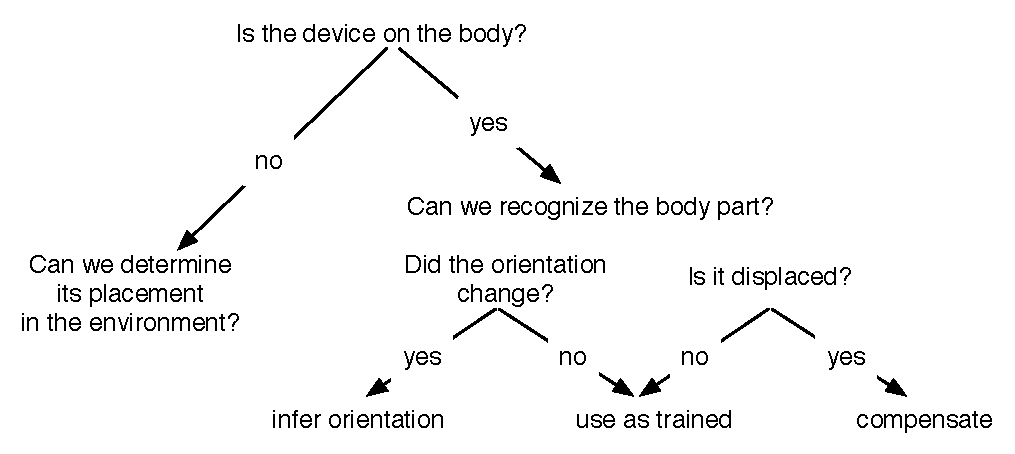
\includegraphics[height=2.3in]{Thesisgraph.pdf}
	\end{center}
 \caption[Thesis overview graph]{Thesis Overview}
\label{fig:graph}
\end{figure}

\begin{figure}[t]
 \begin{center}
 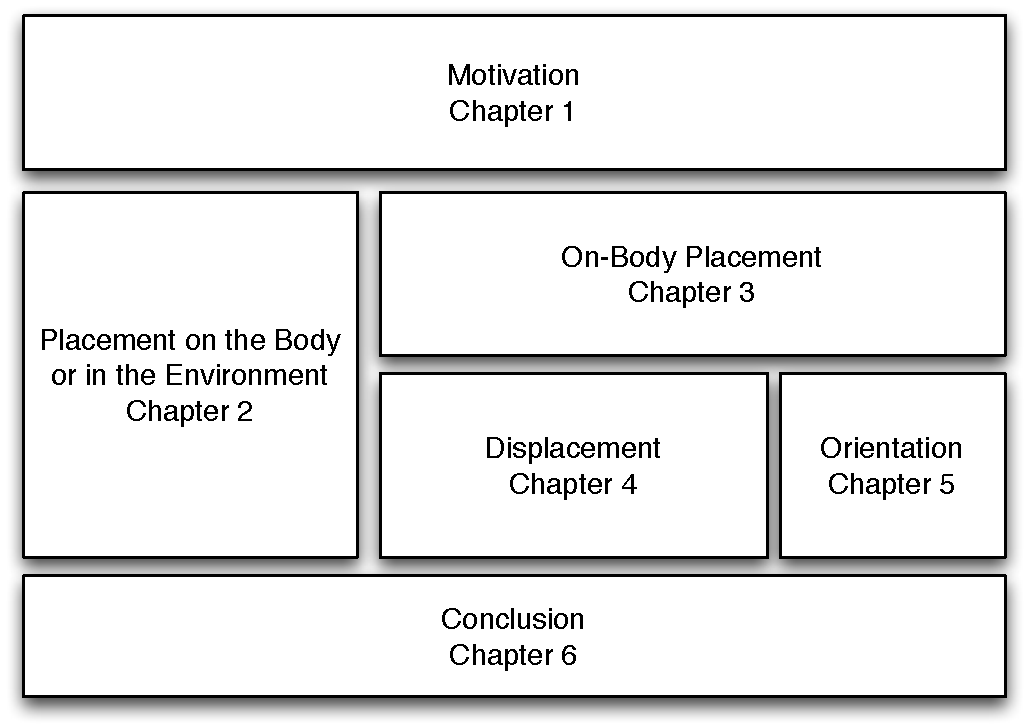
\includegraphics[height=3in]{thesis-overview2.pdf}
	\end{center}
 \caption[Thesis chapters]{Thesis Chapters}
\label{fig:chapters}
\end{figure}

Figure~\ref{fig:graph} gives a detailed description and a categorization of the problems
posed for this work. Coarse variations in sensor signals give information
on whether a device is worn on the body or placed somewhere in the environment. 
Some environmental placements come with their unique sensor signature
depending on the modality. This question is handled in Chapter 2
"Device Placement in the Environment or On-Body". 

If the device is placed on the body, the next logical question is
which body part it is located on.  Impacts on the sensor signals and possible
recognition solutions dealing with this sub-question are handled 
in Chapter 3 "On-Body Placement".

The next two special issues discussed result from long-term deployment.
We deal with translational shifts in Chapter 4 "Displacement" and
orientation changes in Chapter 5 "Orientation".

Figure~\ref{fig:chapters} depicts the chapters.  
The on-body placement chapter is related to the  orientation and displacement chapters.
Therefore, it is recommended to read them in order. 
The conclusion chapter provides a summary of the thesis
and pointers for future work. Table~\ref{PaperContrib} gives an overview 
about the publications used in this thesis and their corresponding chapters.

\begin{table}
 \caption[Publications included in this thesis]{Publications included in this thesis with the respective chapter.}
 \centering
\begin{tabularx}{ \textwidth}{ c|X }
\toprule
 Chapter & Publication \\
 \midrule
 1 %&Kunze, K.,Wagner, F., Kartal, E., Morales Kluge, E., and Lukowicz, P. Does
%Context Matter ? - A Quantitative Evaluation in a Real World
%Maintenance Scenario.\textit{ In Proceedings of the 7th international
% Conference on Pervasive Computing Nara}, Japan, May 11 - 14, 2009.\\
 & Kunze,K., Partridge, K. and Lukowicz, P. Compensating placement
 variations in body worn context recognition systems
 \textit{Submitted to IEEE Pervasive Computing Magazine, 2012}.\\ \midrule

 2 & Kunze, K. and Lukowicz, P. Symbolic object localization through
 active sampling of acceleration and sound signatures.\textit{ In
 Proceedings of the 9th international Conference on Ubiquitous
 Computing}. Innsbruck, Austria, September 16 - 19,
 2007.\\ \midrule 3 & K.~Kunze and P.~Lukowicz. \newblock Using
 acceleration signatures from everyday activities for on-body device
 location. \newblock {\em 11th IEEE International Symposium on
 Wearable Computers}, Sep 2007.\\ &K.~Kunze, P.~Lukowicz,
 H.~Junker, and G.~Troester. \newblock Where am i: Recognizing
 on-body positions of wearable sensors. \newblock {\em LOCA'04:
 International Workshop on Location and Context Awareness }, Jan
 2005.\\ \midrule 4 &Kunze, K. and Lukowicz, P. Dealing with sensor
 displacement in motion-based on-body activity recognition
 systems. In Proceedings of the 10th international conference on
 Ubiquitous computing (UbiComp '08). Seoul, Korea, September,
 2008. \\ \midrule 5 &Kai Kunze, Paul Lukowicz, Kurt Partridge, Bo
 Begole, Which Way Am I Facing: Inferring Horizontal Device
 Orientation from an Accelerometer Signal, \textit{13th IEEE
 International Symposium on Wearable Computers}. Linz, Austria,
 2009.\\ \midrule 6 &Kunze, K., Bahle, G., Lukowicz, P., and
 Partridge, K. Can magnetic field sensors replace gyroscopes in
 wearable sensing applications \textit{In ISWC '10: Proceedings of
 the 2010 11th IEEE International Symposium on Wearable
 Computers}. Seoul, South Korea, 2010.\\ \bottomrule
\end{tabularx}
\label{PaperContrib}
\end{table}


\bibliographystyle{abbrv}
\bibliography{motivation}
